\documentclass[ucs,9pt]{beamer}
\setbeamertemplate{navigation symbols}{}
% remove this line and the "ucs" option to the documentclass when your editor is not utf8-capable
\usepackage[utf8x]{inputenc}    % to make utf-8 input possible
\usepackage[english]{babel}     % hyphenation etc., alternatively use 'german' as parameter
% Template for talks using the Corporate Design of the Freie Universitaet
%   Berlin, created following the guidelines on www.fu-berlin.de/cd by
%   Tobias G. Pfeiffer, <tobias.pfeiffer@math.fu-berlin.de>
% This file can be redistributed and/or modified in any way you like.
%   If you feel you have done significant improvements to this template,
%   please consider providing your modified version to
%   https://www.mi.fu-berlin.de/w/Mi/BeamerTemplateCorporateDesign

\usepackage{amsmath,dsfont,listings}

%%% FU logo
% small version for upper right corner of normal pages
\pgfdeclareimage[height=0.9cm]{university-logo}{FULogo_RGB}
\logo{\pgfuseimage{university-logo}}
% large version for upper right corner of title page
\pgfdeclareimage[height=1.085cm]{big-university-logo}{FULogo_RGB}
\newcommand{\titleimage}[1]{\pgfdeclareimage[height=2.92cm]{title-image}{#1}}
\titlegraphic{\pgfuseimage{title-image}}
%%% end FU logo

% NOTE: 1cm = 0.393 in = 28.346 pt;    1 pt = 1/72 in = 0.0352 cm
\setbeamersize{text margin right=3.5mm, text margin left=7.5mm}  % text margin

% colors to be used
\definecolor{text-grey}{rgb}{0.45, 0.45, 0.45} % grey text on white background
\definecolor{bg-grey}{rgb}{0.66, 0.65, 0.60} % grey background (for white text)
\definecolor{fu-blue}{RGB}{0, 51, 102} % blue text
\definecolor{fu-green}{RGB}{153, 204, 0} % green text
\definecolor{fu-red}{RGB}{204, 0, 0} % red text (used by \alert)

% switch off the sidebars
% TODO: loading \useoutertheme{sidebar} (which is maybe wanted) also inserts
%   a sidebar on title page (unwanted), also indents the page title (unwanted?),
%   and duplicates the navigation symbols (unwanted)
\setbeamersize{sidebar width left=0cm, sidebar width right=0mm}
\setbeamertemplate{sidebar right}{}
\setbeamertemplate{sidebar left}{}
%    XOR
% \useoutertheme{sidebar}

% frame title
% is truncated before logo and splits on two lines
% if neccessary (or manually using \\)
\setbeamertemplate{frametitle}{%
    \vskip-30pt \color{text-grey}\large%
    \begin{minipage}[b][23pt]{80.5mm}%
    \flushleft\insertframetitle%
    \end{minipage}%
}

%%% title page
% TODO: get rid of the navigation symbols on the title page.
%   actually, \frame[plain] *should* remove them...
\setbeamertemplate{title page}{
% upper right: FU logo
\vskip2pt\hfill\pgfuseimage{big-university-logo} \\
\vskip6pt\hskip3pt
% title image of the presentation
\begin{minipage}{11.6cm}
\hspace{-1mm}\inserttitlegraphic
\end{minipage}

% set the title and the author
\vskip14pt
\parbox[top][1.35cm][c]{11cm}{\color{text-grey}\inserttitle \\ \small \insertsubtitle}
\vskip11pt
\parbox[top][1.35cm][c]{11cm}{\small \insertauthor \\ \insertinstitute \\[3mm] \insertdate}
}
%%% end title page

%%% colors
\usecolortheme{lily}
\setbeamercolor*{normal text}{fg=black,bg=white}
\setbeamercolor*{alerted text}{fg=fu-red}
\setbeamercolor*{example text}{fg=fu-green}
\setbeamercolor*{structure}{fg=fu-blue}

\setbeamercolor*{block title}{fg=white,bg=black!50}
\setbeamercolor*{block title alerted}{fg=white,bg=black!50}
\setbeamercolor*{block title example}{fg=white,bg=black!50}

\setbeamercolor*{block body}{bg=black!10}
\setbeamercolor*{block body alerted}{bg=black!10}
\setbeamercolor*{block body example}{bg=black!10}

\setbeamercolor{bibliography entry author}{fg=fu-blue}
% TODO: this doesn't work at all:
\setbeamercolor{bibliography entry journal}{fg=text-grey}

\setbeamercolor{item}{fg=fu-blue}
\setbeamercolor{navigation symbols}{fg=text-grey,bg=bg-grey}
%%% end colors

%%% headline
\setbeamertemplate{headline}{
\vskip4pt\hfill\insertlogo\hspace{3.5mm} % logo on the right

\vskip6pt\color{fu-blue}\rule{\textwidth}{0.4pt} % horizontal line
}
%%% end headline

%%% footline
\newcommand{\footlinetext}{\insertshortinstitute, \insertshorttitle, \insertshortdate}
\setbeamertemplate{footline}{
\vskip5pt\color{fu-blue}\rule{\textwidth}{0.4pt}\\ % horizontal line
\vskip2pt
\makebox[123mm]{\hspace{7.5mm}
\color{fu-blue}\footlinetext
\hfill \raisebox{-1pt}{\usebeamertemplate***{navigation symbols}}
\hfill \insertframenumber}
\vskip4pt
}
%%% end footline

%%% settings for listings package
\lstset{extendedchars=true, showstringspaces=false, basicstyle=\footnotesize\sffamily, tabsize=2, breaklines=true, breakindent=10pt, frame=l, columns=fullflexible}
\lstset{language=Java} % this sets the syntax highlighting
\lstset{mathescape=true} % this switches on $...$ substitution in code
% enables UTF-8 in source code:
\lstset{literate={ä}{{\"a}}1 {ö}{{\"o}}1 {ü}{{\"u}}1 {Ä}{{\"A}}1 {Ö}{{\"O}}1 {Ü}{{\"U}}1 {ß}{\ss}1}
%%% end listings  % THIS is the line that includes the FU template!

\usepackage{arev,t1enc} % looks nicer than the standard sans-serif font
% if you experience problems, comment out the line above and change
% the documentclass option "9pt" to "10pt"

% image to be shown on the title page (without file extension, should be pdf or png)
\titleimage{mi-bildbalken}
\title[Para Sort] % (optional, use only with long paper titles)
{Paralleles Sortierung}

%\subtitle
%{Include Only If Paper Has a Subtitle}

\author[] % (optional, use only with lots of authors)
{Björn Rathjen \and Patrick Winterstein}
% - Give the names in the same order as the appear in the paper.

\institute[FU Berlin] % (optional, but mostly needed)
{Freie Universität Berlin}

\date[ProSem Algo]
{Proseminar Algorithmen, SS14}

%\subject{Theoretical Computer Science}
% This is only inserted into the PDF information catalog. Can be left
% out.

% you can redefine the text shown in the footline. use a combination of
% \insertshortauthor, \insertshortinstitute, \insertshorttitle, \insertshortdate, ...
\renewcommand{\footlinetext}{\insertshortinstitute, \insertshorttitle, \insertshortdate}

\AtBeginSection[]
{
\begin{frame}<beamer>
	\tableofcontents[currentsection,hideothersubsubsections,hideothersubsections]
\end{frame}
}
\begin{document}
%Titelblatt
%1
\begin{frame}[plain]
  \titlepage
\end{frame}
 
%Inhaltsverzeichnis
%2
\begin{frame}{Inhalt}
  \tableofcontents[hideallsubsubsections,allowframebreaks] %currentsection,hideallsubsections,hideallsubsubsections
  % You might wish to add the option [pausesections]
\end{frame}


% Motivation
%3
\section{Motivation}

%4  
\begin{frame}{Motivation : Allgemein}
Sortieren \\
    ist Grundlage für :
    \begin{itemize}
        \item Suche
        \item (Sortierung)
        \begin{itemize}
            \item Listen
            \item Wörterbücher
            \item ... 
        \end{itemize}
        \item Ist dies auch effektiver / in Hardware möglich ?
    \end{itemize}
\end{frame}

%5
\section{Grundlage des Sortierens}
\subsection{Komparator}

%6
\begin{frame}{Aufbau}
    \begin{minipage}[c]{14.5cm}
    		\begin{minipage}[c]{5cm}
        		\begin{itemize}
            		\item 2 Eingänge
	            	\item vergleichender Baustein
    		        	\item 2 Ausgänge
        		\end{itemize}
	    \end{minipage}
%    		\hfill
		\begin{minipage}[c]{5cm}
			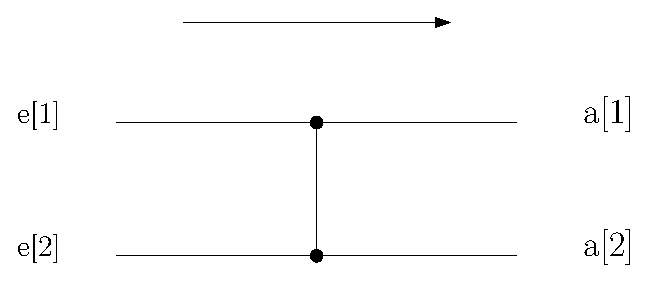
\includegraphics[scale=0.5]{Komparator1.eps}
	 	\end{minipage}
    \end{minipage}
\end{frame}

%Pseudocode
%7
\begin{frame}[fragile]{Vergleichender Baustein (ii)}
\begin{center}
\begin{lstlisting}[laguage={inform},tabsize=4,numbers=left]
    void comp(chan in1, in2, out1, out2 Comparer{}){
        a := <- in1;
        b := <- in2;
        
        if (a < b){
            out1 <- a;
            out2 <- b;
            return void;
        }
        out1 <- b;
        out2 <- a;
        return void;
    }
\end{lstlisting}
\end{center}
\end{frame}

%8
\section{Sortiernetzwerk}
\subsection{Aufbau}

%9
\begin{frame}{Erweiterung : Aufbau , Aufgabe}
\uncover<1-> { Aufbau :\\ \begin{itemize}
        \item mehrere Eingabeleitungen (gleiche Anzahl an Ausgabeleitungen)
        \item mehrere vergleichende Schritte
    \end{itemize}}
\uncover<2-> {Aufgabe :\\
        \begin{itemize}
            \item Resultat soll sortierte Ausgabe sein
            \end{itemize}
            }
\uncover<3-> {grundlegendes Prinzip :
        \begin{itemize}
            \item intuitiver Einsatz von Vergleichen
            \item Schrittweises sortieren
        \end{itemize}}
\end{frame}

%10
\subsubsection*{naiver Ansatz}

%11
\begin{frame}{naiv : grundlegendes Prinzip}
\begin{minipage}[l]{2cm}
Input
\end{minipage}
\begin{minipage}[c]{7cm}
\begin{center}
    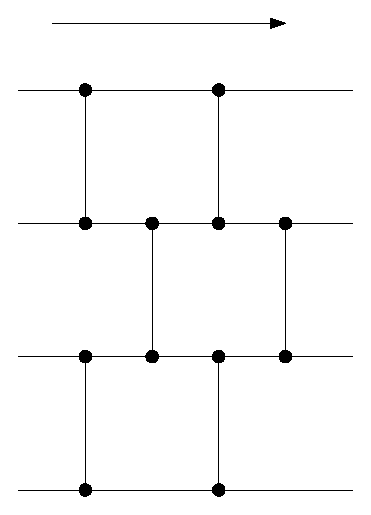
\includegraphics[scale=0.8]{bild2Komparatornetzwerk.eps}
\end{center}
\end{minipage}
\begin{minipage}[r]{2cm}
Output
\end{minipage}
\end{frame}

%12
\begin{frame}{Demonstration}
\begin{center}
   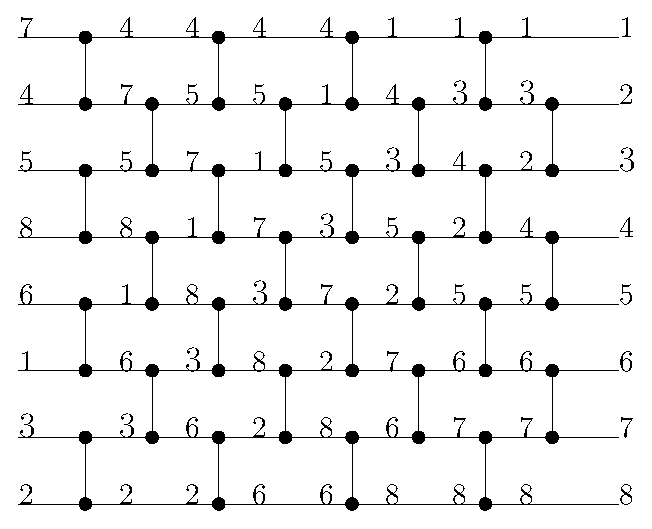
\includegraphics[scale=0.8]{bild2beispiel.eps}\\
\uncover<2-> {Das Zahlenbeispiel funktioniert, aber funktioniert auch jedes andere ?}\\
  \end{center}
\end{frame}

%13
\subsection{Korrektheit}
\begin{frame}{0,1-Prinzip}
\vfill
\uncover<1-> {
\begin{center}
\begin{minipage}[c]{9cm}
Lemma: \\
Wenn es eine Folge A gibt, die ein Sor\-tier\-netz\-werk nicht sortiert, so existiert auch eine 0,1-Folge, die von diesem Netzwerk nicht sortiert wird.
\end{minipage}
\vfill
\end{center}
}
\begin{itemize}
\uncover<2-> { \item Führen einen Beweis durch Widerspruch \\}
\uncover<3-> { \item d.h : Wenn ein Algorithmus eine Eingabefolge nicht sortiert, so sortiert er alle 0,1-Folgen. }
\uncover<4-> { \item somit ist das Ziel eine 0,1-Folge zu finden, die nicht sortiert wird}
\end{itemize} 
\end{frame}

%14
\begin{frame}{Beweis : 0,1-Prinzip}
\begin{proof}
\begin{itemize}
\item benötigen folgendes
\begin{itemize}
\uncover<2-> {\item Eingabefolge $E \; = \; e_0 … e_N$}
\uncover<3-> {\item sortierte Folge $S\; = \; s_0 … s_N$}
\uncover<4-> {\item unsortierte Ausgabefolge von E $U \; = \; u_0 … u_N$}
\uncover<5-> {\item k : (kleinster) Index an dem $u_k \neq s_k$}
\end{itemize}
\uncover<6-> {\item dann gilt :
\begin{enumerate}
\item[(1)] $u_i = s_i \;\;\forall \;0 \leq i < k$ 
% alle Werte vor k sind sortiert 
% muss existieren, da u unsortiert ist
\uncover<7-> {\item[(2)] $u_r = s_k \;\; \text{mit : }r>k  $}
% es gibt also ein Element das in der Folge danach steht und dem sortierten Elemelnt entspricht
\end{enumerate}}
\end{itemize}
\end{proof}
\end{frame} 

%15
\begin{frame}
\begin{proof}
\begin{itemize}
\item 
    man kann jede Zahlenfolge durch eine 0,1 Folge repräsentieren\\
    Konstante c $(\text{hier : }c = s_k)$ und Zahlenfolge E mit den Elementen $e_i$\\
    $$
    f(e) = \begin{cases} 0 , & if \;\; e_i \leq s_k \\
    1 , & if \;\; e_i > s_k
    \end{cases}$$
\uncover<2-> {\item Ausgabe muss also wie folgt aussehen 
$$ 00 …… 01{\uncover <3-> {_k}}…0_{\uncover <3-> {_r}} …$$}
\uncover<4-> {\item[$\Rightarrow$] 0,1-Folge ist nicht sortiert}
\uncover<5-> {\item[$\Rightarrow$] Widerspruch zur Annahme }
\end{itemize}
\end{proof}
\end{frame}

%16
\begin{frame}{0,1- Beispiel}
\uncover<1-> {
\begin{center}
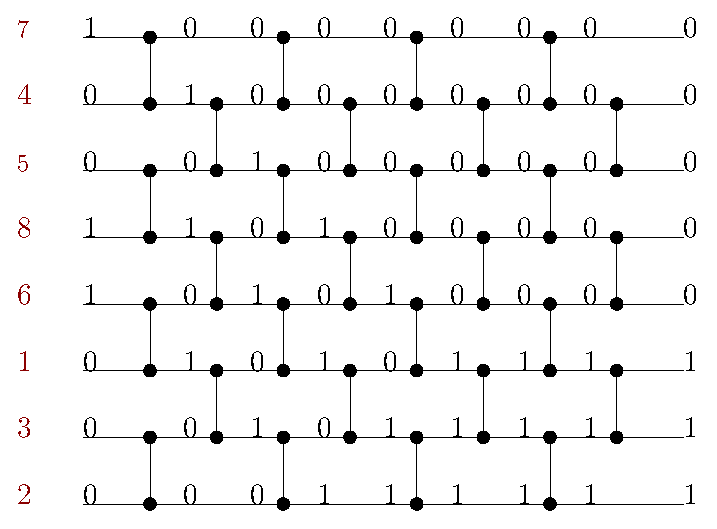
\includegraphics[scale=0.8]{01beispiel.eps}
\end{center}
}
%Bild letzte Komparatorebene weglassen
%\uncover<2-> {\begin{center} {\color{green}Beispiel an der Tafel ?}\end{center} }
\end{frame}

%17
\begin{frame}{0,1-Prinzip}
Vorteile des 0,1-Prinzips : 
\begin{itemize}
\item einfach 
	\begin{itemize}
		\item sauberer Testcode
		\item Sicherheit
	\end{itemize}
\item Anzahl der Testfälle sinkt \\ 
$$  W^n\rightarrow 2^n $$
\end{itemize}
\end{frame}

%18
\begin{frame}{Bubblesort im Komparatornetz}
	\begin{center}
	    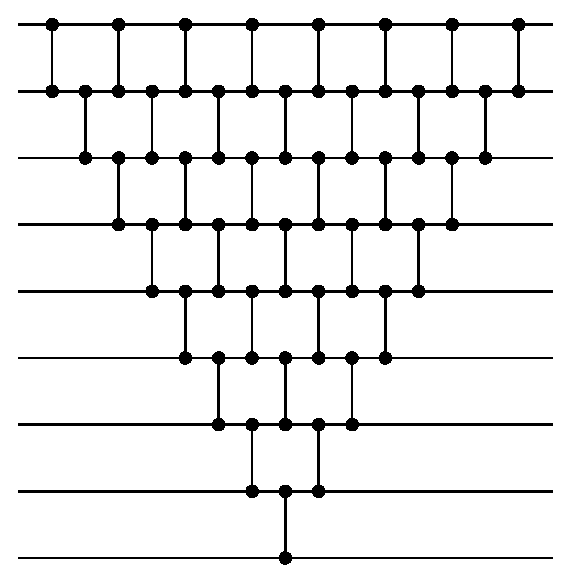
\includegraphics[scale=0.65]{bubblesort.eps}
	\end{center}
\end{frame}

%19
\begin{frame}{Softwaresortieren im Hardwarenetz}
\hspace{1cm} Quicksort \hspace{4cm} Mergesort
    \begin{center}
    		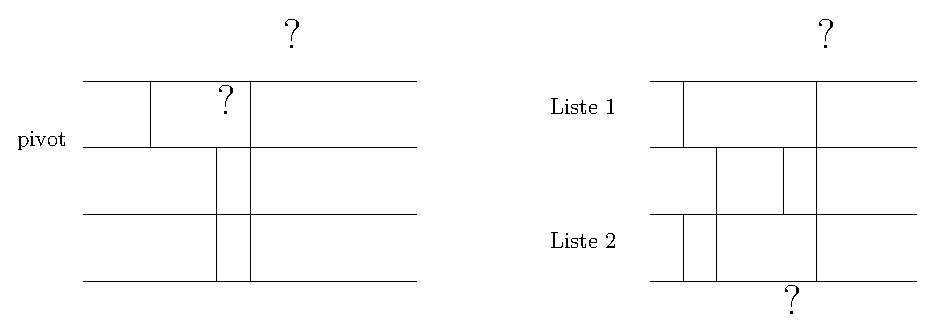
\includegraphics[scale=0.65]{mergesort.eps}
    		%Zeichnung 1 Pivot ist nicht auffindbar
    		%Zeichnung 2 wo war das größere Element vorher 
    		%			welcher Vergleich muss nun gemacht werden
\end{center}     
\uncover<2-> {Quicksort : wo ist das Pivot Element ?\\ Mit welchem Element müssen wir nun vergleichen?}\\
\uncover<3-> {Mergesort : Wo ist nun das größte Element ? \\welcher Vergleich kommt nun?)}
\end{frame}

%20
\subsection*{Aufbau eines effektieveren Netzwerks}
%Einsatzorte
\begin{frame}{effektiveres Netzwerk}
\uncover<2-> {Aufgabe :
            \begin{itemize}
                \item Resultat soll sortierte Ausgabe sein
                \item \alert{soll effizient sein}
            \end{itemize}}
\uncover<3-> {grundlegendes Prinzip :
            \begin{itemize}
                \item intuitiver Einsatz von Vergleichen
                \item[]\alert{+ Einbezug von Teile und Herrsche}
                % mh sehr leere Folien
            \end{itemize}}
\end{frame}

\subsection{Biton-Sortierer}
%21
\begin{frame}{Übertragung auf Komparatornetzwerk}
\begin{center}
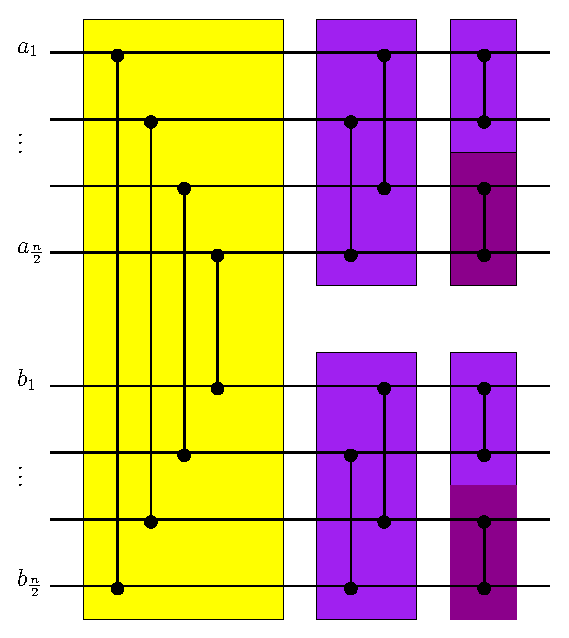
\includegraphics[scale=0.6]{bitonmischer.eps}
\end{center}
\end{frame}

%22
\begin{frame}{Bitonmischer}
Ablauf :
\begin{itemize}
\item sortiert / mischt Eingabelisten
	\begin{itemize}
	\item untere Hälfte alle größer als in oberer
	\end{itemize}
\item rekursiv die kleineren Listen 
\item Resultat eine Sortierte Liste
\end{itemize}
\end{frame}

%23
\begin{frame}{Biton -Sortierer : Aufbau}
    \begin{center}
    		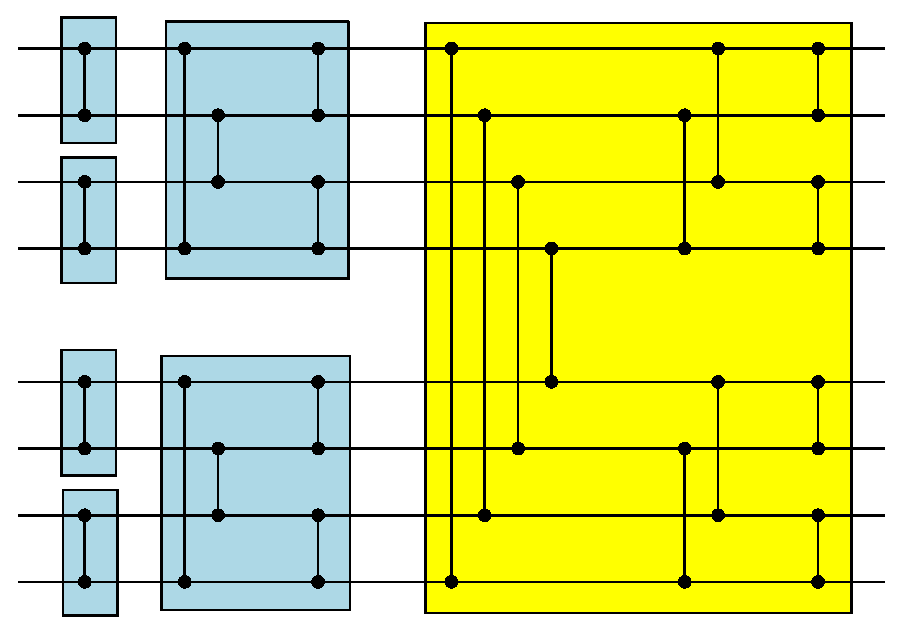
\includegraphics[scale=0.6]{biton2.eps}
    \end{center}
    \uncover<2-> { Beispiel an der Tafel}
\end{frame}


%24
\subsection{Odd-Even-Mergesort}
\begin{frame}{odd even sort}
\uncover<1-> {Ablauf :
\begin{itemize}
\uncover<2-> {\item Voraussetzung : bekommen zwei sortierte Listen}
\uncover<3-> {\item trennen in geraden und ungeraden Index}
\uncover<4-> {\item fassen a(even) b(odd) = c und a(odd) b(even) = d zusammen (Resultat wird rekursiv sortiert)}
\uncover<5-> {\item sortierte c und d werden indexweise verschachtelt}
\uncover<6-> {\item aufeinander folgende Paare werden verglichen und in richtige Reihenfolge gebracht}
\end{itemize}}
\end{frame}

%25
\begin{frame}{Beispiel : Odd-Even-Mergesort}
Beispiel : \\
\begin{itemize}
%zwei sortierte Listen 
\item[] $$ A = 2,3,4,8 $$
\item[] $$ B = 1,5,6,7 $$
%indexweise aufteilen zusammenbringen und sortieren
\uncover<2-> {\item[] $$ A_e = 2,4 \;\;\; B_o = 5,7 \;\;\; \Rightarrow \;\;\; C= 2,4,5,7 $$}
\uncover<3-> {\item[] $$ A_o = 3,8 \;\;\; B_e = 1,6 \;\;\; \Rightarrow \;\;\; D = 1,3,6,8 $$}
%verschachteln
\uncover<4-> {\item[] nach dem Verschachteln $$ 2,1,4,3,5,6,7,8$$}
%nebeneinanderstehende vergleichen
\uncover<5-> {\item[] Resultat : $$1,2,3,4,5,6,7,8$$}
\end{itemize}
\end{frame}

%26
\begin{frame}{Sortiernetzwerk}
\begin{center}
\includegraphics[scale=0.65]{oddeven1.eps}
\end{center}
\end{frame}

%27
\begin{frame}{Wieso funktioniert das?}
\begin{itemize}
\item Veranschaulichung mit dem 0,1-Pinzip
	\begin{itemize}
		% Illustration an der Tafel
		% listen teilen ineinander 0 und 1 
		% Verschachtelung legt diese zusammen
		% nur aufeinanderfolgende müssen verglichen werden weil i+2 schon sortiert ist
		\item gleichmäßiges Aufteilen von Nullen und Einsen
		\item somit alle nah beieinander
	\end{itemize}

\end{itemize}
\end{frame}

%28
\section{Laufzeit}
\subsection{Herleitung}

%29
\begin{frame}{Herleitung der Laufzeit}
\begin{center}
\begin{tabular}{c|c}
%eventuell noch 2^0
% paralleles zeigen an der Tafel / folie 
Länge der Eingabe & Anzahl der Schritte \\
\hline \\
\uncover<1-> {$2^1$} & \uncover<2-> { $1$}\\
\uncover<3-> {$2^2$} & \uncover<4-> { $1 + 2$}\\
\uncover<5-> {$2^k$}& \uncover<6-> { $1 + 2 + 3 + … + k-1 + k  = \sum_{i=1}^k i$}\\
\uncover<7-> {{\color{gray}(kleiner Gauss)}} & \uncover<8-> {$ =\frac{1}{2}\cdot k \cdot (k+1) $} \\
\uncover<9-> {{\color{gray}$(k = log_2 n)$}} &\uncover<10-> {$\Rightarrow \frac{1}{2}\; \cdot\;\log_2 n \;\; (\log_2 n\;+\;1)$} \\
\end{tabular}
\end{center}
\end{frame}

%30
\subsection{Vergleich mit Software sortieren}
\begin{frame}{Vergleich zu bekannten Softwareansätzen}
	\begin{itemize}
		\item Schritte gegen Vergleiche
			\begin{itemize}
				\item in jedem Schritt $\frac{n}{2}$ Komparatoren benötigt 
				\item[] $\frac{n}{2}\;\cdot \left( \frac{1}{2} \cdot\;\log_2 n \;\; (\log_2 n\;+\;1)\right)$ 
				\item 1 Vergleicher bei Software benötigt
				\item Laufzeit konstant
			\end{itemize}
	 	\item Abhängigkeit von der Eingabe
	 	\item Bezug zum vorherigen Vergleich
	 	\item die andere Laufzeiten
\end{itemize}
\begin{center}
	 	\begin{tabular}{c|c|c|c}
	 	Algorithmus & \multicolumn{3}{c}{Laufzeit } \\ \hline
	 	 & best & worst & \uncover<2-> {avarage / normiert}\\ \cline{2-4}
	 	 & & & \\
	 	 Bubblesort & O($n$) & O($n^2$)& \uncover<2-> {}\\
	 	 Mergosort & \multicolumn{2}{c|}{O$(n \log n)$} &  \uncover<2-> {O$(n \log n )$}\\
	 	 Quicksort & O($n\log n$) & O($n^2$) & \uncover<2-> {O$(n \log n) $}\\
	 	 Netzwerk & \multicolumn{2}{c|}{O$(\log^2n)$} & \uncover<2-> {O$(n\log^2n)$} \\
	 	\end{tabular}
	 	\end{center}
\end{frame}

%31
\section{Zusammenfassung}
\begin{frame}{Zusammenfassung}
paralleles Sortieren ist
\begin{itemize}
  \item schnell 
  \item aber erfordert mehr Ressourcen 
  \item problemabhängige Lösung (Eingabegröße)
\end{itemize}
\end{frame}

%32
\section{Ausblick}
\begin{frame}{Ausblick}
\begin{itemize}
\item aks-Netzwerke ($O(c \cdot n \cdot \log n)$
\item $\rightarrow$ Hypercubes
\item Paketrouting 
%\item Simulation von Maschinenmodellen 
\item u.v.m.
\end{itemize}
\end{frame}

%33
\subsection{Anhang}
\appendix
\section<presentation>*{\appendixname}
\subsection<presentation>*{For Further Reading}

\begin{frame}[allowframebreaks]
  \frametitle<presentation>{For Further Reading}
    
  \begin{thebibliography}{10}
    
  \beamertemplatebookbibitems
  % Start with overview books.

  \bibitem{}
    \newblock {\em Taschenbuch der Algorithmen}.
    \newblock Springer Verlag , 2008.
    
  \bibitem{Author1990}
    Tom Leighton.
    \newblock {\em Einführung in Parallele Algorithmen und Architekturen}{\\Gitter, Bäume und Hypercubes}.
    \newblock Thomsom Publisching , 1997.
    \newblock 3-8266-0248-X
 
    
  \beamertemplatearticlebibitems
	\bibitem{Sortieralgorithmen}
		\newblock Laufzeiten Sortieralgorithmen
		\newblock {www.wikipedia.de}  
  
  % Followed by interesting articles. Keep the list short. 

  \bibitem{0,1-Prinzip}
%    \href{http://www.iti.fh-flensburg.de/lang/algorithmen/sortieren/networks/nulleins.htm}
    \newblock Alternativer Ansatz zum Beweis des 0,1-Prinzip
    \newblock {http://www.iti.fh-flensburg.de/lang/algorithmen/sortieren/networks/nulleins.htm}
    
  \end{thebibliography}
\end{frame}

%35
\begin{frame}{Ende}
    Fragen, Anregungen?\\
\end{frame}

\end{document}
%end